\documentclass[tikz, border=14pt]{standalone}
\usepackage{tikz}
\usetikzlibrary{arrows.meta, backgrounds, calc}
\usepackage{amsmath}

\definecolor{cA}  {RGB}{ 74,144,226}
\definecolor{cB}  {RGB}{174, 36,206}
\definecolor{cC}  {RGB}{230,158, 28}
\definecolor{cVis}{RGB}{150,178,205}
\definecolor{cMsk}{RGB}{210,212,218}
\definecolor{cBlk}{RGB}{178,182,190}
\definecolor{cP1} {RGB}{194, 65, 12}
\definecolor{cP2} {RGB}{100, 40,200}

\newcommand{\sq}[4]{%
  \fill[#4, draw=white, line width=0.65pt]
    (#1,#2) rectangle ({#1+#3},{#2+#3});}

\begin{document}
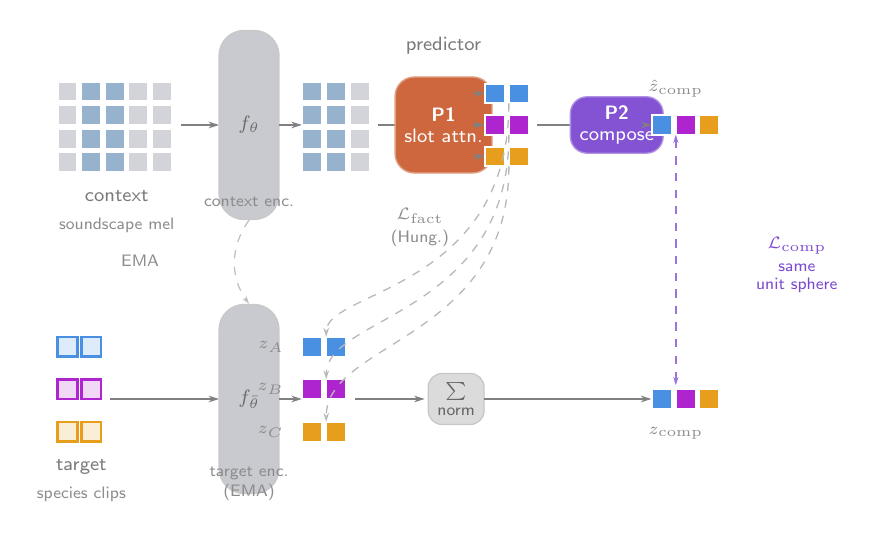
\begin{tikzpicture}[
  enc/.style={rectangle, rounded corners=9pt,
    fill=cBlk!72, draw=gray!42, line width=0.50pt,
    minimum width=0.76cm, minimum height=2.40cm,
    font=\fontsize{7.5}{9}\selectfont\sffamily, text=black!58, align=center},
  p1blk/.style={rectangle, rounded corners=7pt,
    fill=cP1!80, draw=cP1!50, line width=0.50pt,
    minimum width=0.76cm, minimum height=1.22cm,
    font=\fontsize{7}{8.5}\selectfont\sffamily, text=white, align=center},
  p2blk/.style={rectangle, rounded corners=6pt,
    fill=cP2!80, draw=cP2!50, line width=0.48pt,
    minimum width=0.74cm, minimum height=0.58cm,
    font=\fontsize{7}{8.5}\selectfont\sffamily, text=white, align=center},
  sumnorm/.style={rectangle, rounded corners=5pt,
    fill=gray!28, draw=gray!44, line width=0.45pt,
    minimum width=0.70cm, minimum height=0.56cm,
    font=\fontsize{6.5}{8}\selectfont\sffamily, text=black!60, align=center},
  fw/.style={-{Stealth[length=3.8pt,width=2.4pt]}, line width=0.55pt, black!50},
  lcon/.style={-{Stealth[length=3.2pt,width=2.0pt]},
               dashed, line width=0.48pt, gray!55},
  lcomp/.style={{Stealth[length=3.0pt,width=1.9pt]}-{Stealth[length=3.0pt,width=1.9pt]},
                dashed, line width=0.50pt, cP2!65},
  ann/.style={font=\fontsize{7.5}{9}\selectfont\sffamily, text=black!52, align=center},
  smol/.style={font=\fontsize{6}{7.5}\selectfont\sffamily, text=black!45, align=center},
]

\def\ps{0.25}
\def\pd{0.30}

%% ── Key computed x positions ──────────────────────────────────────────────
%% Mel grid  : x=[0, 1.50]       (5 cols)
%% f_θ center: x=2.43
%% Tok grid  : x=[3.11, 4.01]    (3 cols)
%% P1 center : x=4.90
%% K slots   : x=[5.43, 6.03]    (2 cols), x-center = 5.73
%% P2 center : x=7.10
%% z_hat     : x=[7.55, 8.45]    (3 patches at pd=0.30)
%% L_comp    : x-center = 8.00
%% ─────────────────────────────────────────────────────────────────────────

%% ══════════════════════════════════════════════════════════════════
%% CONTEXT PATH  (top)
%% ══════════════════════════════════════════════════════════════════

%% 1. Mel spectrogram  5×4, cols 1-2 visible
\foreach \c in {0,...,4}{
  \foreach \r in {0,...,3}{
    \pgfmathsetmacro\px{0.00+\c*\pd}
    \pgfmathsetmacro\py{3.30+\r*\pd}
    \ifnum\c=1 \sq{\px}{\py}{\ps}{cVis}
    \else\ifnum\c=2 \sq{\px}{\py}{\ps}{cVis}
    \else          \sq{\px}{\py}{\ps}{cMsk}
    \fi\fi}}
\node[ann,  below=3pt]  at ({2.5*\pd}, 3.30) {context};
\node[smol, below=13pt] at ({2.5*\pd}, 3.30) {soundscape mel};

\draw[fw] ({5*\pd+0.06}, 3.90) -- (2.05, 3.90);

%% 2. Context encoder
\node[enc] (ec) at (2.43, 3.90) {$f_\theta$};
\node[smol, below=5pt] at (2.43, 3.28) {context enc.};
\draw[fw] (2.81, 3.90) -- (3.10, 3.90);

%% 3. Token grid  3×4
\foreach \c in {0,...,2}{
  \foreach \r in {0,...,3}{
    \pgfmathsetmacro\px{3.11+\c*\pd}
    \pgfmathsetmacro\py{3.30+\r*\pd}
    \ifnum\c=2 \sq{\px}{\py}{\ps}{cMsk}
    \else      \sq{\px}{\py}{\ps}{cVis}
    \fi}}
\draw[fw] ({3.11+3*\pd+0.06}, 3.90) -- (4.52, 3.90);

%% 4. P1 Slot Attention
\node[p1blk] (p1) at (4.90, 3.90) {\textbf{P1}\\[-1pt]slot attn.};
\node[ann, above=5pt] at (4.90, {3.30+4.0*\pd}) {predictor};

%% Fan-out P1 → 3 slot rows (short horizontal arrows)
\draw[fw] (5.28, 4.30) -- (5.42, 4.30);
\draw[fw] (5.28, 3.90) -- (5.42, 3.90);
\draw[fw] (5.28, 3.50) -- (5.42, 3.50);

%% 5. K slot squares  (2 wide × 1 tall, 3 rows; centers at y=4.30, 3.90, 3.50)
%% slot A: y_bottom=4.175, slot B: y_bottom=3.775, slot C: y_bottom=3.375
\foreach \c in {0,1}{ \sq{5.43+\c*\pd}{4.175}{\ps}{cA} }
\foreach \c in {0,1}{ \sq{5.43+\c*\pd}{3.775}{\ps}{cB} }
\foreach \c in {0,1}{ \sq{5.43+\c*\pd}{3.375}{\ps}{cC} }

%% Gather: K slots → P2
\draw[fw] ({5.43+2*\pd+0.06}, 3.90) to[out=0,in=180] (6.73, 3.90);

%% 6. P2 Compose
\node[p2blk] (p2) at (7.10, 3.90) {\textbf{P2}\\[-1pt]compose};
\draw[fw] (7.47, 3.90) -- (7.54, 3.90);

%% 7. z_hat_comp  (3-patch strip cA|cB|cC, centered vertically on y=3.90)
\sq{7.55}{3.775}{\ps}{cA}
\sq{7.55+\pd}{3.775}{\ps}{cB}
\sq{7.55+2*\pd}{3.775}{\ps}{cC}
\node[smol, above=3pt] at ({7.55+\pd}, {3.775+\ps})
  {$\hat{z}_{\mathrm{comp}}$};

%% ══════════════════════════════════════════════════════════════════
%% TARGET PATH  (bottom)
%% ══════════════════════════════════════════════════════════════════

%% 1. Species clip thumbnails
\foreach \clipy/\clipcol in {0.96/cA, 0.42/cB, -0.12/cC}{
  \foreach \c in {0,1}{
    \pgfmathsetmacro\px{0.00+\c*\pd}
    \fill[\clipcol!18, draw=\clipcol, line width=0.9pt]
      (\px,\clipy) rectangle (\px+\ps,\clipy+\ps);}}
\node[ann,  below=3pt]  at (\pd, -0.12) {target};
\node[smol, below=13pt] at (\pd, -0.12) {species clips};

\draw[fw] ({2*\pd+0.06}, 0.42) -- (2.05, 0.42);

%% 2. Target encoder (EMA)
\node[enc] (et) at (2.43, 0.42) {$f_{\bar\theta}$};
\node[smol, below=5pt] at (2.43, -0.14) {target enc.\\(EMA)};

%% EMA arc  f_θ → f_θ̄
\draw[-{Stealth[length=2.8pt,width=1.8pt]}, dashed, line width=0.44pt, gray!50]
  (ec.south) to[bend right=36] (et.north);
\node[smol, left=2pt] at (1.48, 2.18) {EMA};

\draw[fw] (2.81, 0.42) -- (3.10, 0.42);

%% 3. z_A, z_B, z_C  (2 wide × 1 tall each)
%%    x=[3.11, 3.71];  y_bottoms: 0.96, 0.42, -0.12
\foreach \c in {0,1}{ \sq{3.11+\c*\pd}{0.96}{\ps}{cA} }
\foreach \c in {0,1}{ \sq{3.11+\c*\pd}{0.42}{\ps}{cB} }
\foreach \c in {0,1}{ \sq{3.11+\c*\pd}{-0.12}{\ps}{cC} }
%% Labels to the LEFT of each square
\node[smol, left=3pt] at (3.10, 1.085) {$z_A$};
\node[smol, left=3pt] at (3.10, 0.545) {$z_B$};
\node[smol, left=3pt] at (3.10, 0.005) {$z_C$};

%% Gather: z latents → ∑ norm
\draw[fw] ({3.11+2*\pd+0.06}, 0.42) to[out=0,in=180] (4.66, 0.42);

%% 4. ∑ norm
\node[sumnorm] (sn) at (5.06, 0.42) {$\textstyle\sum$\\[-1pt]norm};

%% Long arrow ∑norm → z_comp  (same x-column as z_hat_comp)
\draw[fw] (5.42, 0.42) -- (7.54, 0.42);

%% 5. z_comp  (same 3-patch strip — same representation space)
\sq{7.55}{0.295}{\ps}{cA}
\sq{7.55+\pd}{0.295}{\ps}{cB}
\sq{7.55+2*\pd}{0.295}{\ps}{cC}
\node[smol, below=3pt] at ({7.55+\pd}, 0.295) {$z_{\mathrm{comp}}$};

%% ══════════════════════════════════════════════════════════════════
%% L_comp:  z_hat_comp ↔ z_comp   (vertical double arrow, same column)
%% ══════════════════════════════════════════════════════════════════

\pgfmathsetmacro\lcx{7.55+\pd}           %% x = centre patch of strip
\draw[lcomp] (\lcx, 3.775) -- (\lcx, {0.295+\ps+0.05});
\node[smol, right=5pt, text=cP2!85] at ({7.55+3*\pd+0.12}, 2.12)
  {$\mathcal{L}_{\mathrm{comp}}$\\[1pt]same\\[-1pt]unit sphere};

%% ══════════════════════════════════════════════════════════════════
%% L_factored:  K slots ↔ {z_A, z_B, z_C}   (Hungarian)
%%
%% Arrows route THROUGH THE GAP between context and target paths:
%%   bottom of each slot → arc down-left through gap → top of target latent
%% This avoids threading through P2 or z_hat.
%% ══════════════════════════════════════════════════════════════════

%% slot x-centre = 5.73;  target x-centre = 3.41
%% Slot A bottom y=4.175 → z_A top y=0.96+0.25=1.21   (gap mid y≈1.80)
\draw[lcon]
  (5.73, 4.175)
  .. controls (5.73, 1.80) and (3.41, 1.80) ..
  (3.41, 1.21);

%% Slot B bottom y=3.775 → z_B top y=0.42+0.25=0.67   (gap mid y≈1.48)
\draw[lcon]
  (5.73, 3.775)
  .. controls (5.73, 1.48) and (3.41, 1.48) ..
  (3.41, 0.67);

%% Slot C bottom y=3.375 → z_C top y=-0.12+0.25=0.13   (gap mid y≈1.16)
\draw[lcon]
  (5.73, 3.375)
  .. controls (5.73, 1.16) and (3.41, 1.16) ..
  (3.41, 0.13);

%% L_fact label: centre of arc bundle in the gap
\node[smol, text=black!45] at (4.60, 2.60)
  {$\mathcal{L}_{\mathrm{fact}}$\\[1pt](Hung.)};

\end{tikzpicture}
\end{document}
